\section{Outlier and Outlier Analysis}


\begin{frame}
  \frametitle{What are Outliers?}
  \begin{itemize}
  \item \textbf{Outlier}:
    \begin{itemize}
    \item A data object that \textbf{\color{airforceblue}deviates significantly} from the normal objects as if it were generated by a different mechanism.
      \begin{itemize}
      \item I.e. unusual credit card purchase, or in Sports: Michael Jordon, Wayne Gretzky, $\ldots$
      \end{itemize}
    \end{itemize}
  \item \textbf{Outliers are different from noise.}
    \begin{itemize}
    \item Noise is a random error or variance in a measured variable.
    \item Noise should be removed before outlier detection.
    \end{itemize}
  \item \textbf{Outliers are interesting.}
    \begin{itemize}
    \item They violate the mechanism that generates the normal data.
    \end{itemize}
  \item \textbf{Outlier detection vs. novelty detection:}
    \begin{itemize}
    \item Early stage: outlier; but later merged into the model.
    \end{itemize}
  \end{itemize}
\end{frame}


\begin{frame}
  \frametitle{Where to use it?}
  \begin{itemize}
  \item \textbf{Applications}:
    \begin{itemize}
    \item Credit-card-fraud detection.
    \item Telecom-fraud detection.
    \item Customer segmentation.
    \item Medical analysis.
    \end{itemize}
  \end{itemize}
\end{frame}


\begin{frame}
  \frametitle{Types of Outliers}
  \begin{itemize}
  \item Three kinds: global, contextual, and collective outliers
  \item \textbf{Global} outlier (or \textbf{\color{airforceblue}point anomaly}):
    \begin{itemize}
    \item Significantly deviates from the rest of the data set.
      \begin{itemize}
      \item I.e. intrusion detection in computer networks.
      \end{itemize}
    \item Issue: Find an appropriate measurement of deviation.
    \end{itemize}
  \item \textbf{Contextual} outlier (or conditional outlier):
    \begin{itemize}
    \item Deviates significantly based on a selected context.
      \begin{itemize}
      \item I.e.  $80^{\circ}$F in Urbana outlier? (Depending on summer or winter).
      \end{itemize}
    \item Attributes of data objects divided into two groups:
      \begin{itemize}
      \item \textbf{Contextual attributes}: define the context, e.g., time \& location.
      \item \textbf{Behavioral attributes}: characteristics of the object, used in outlier evaluation, e.g., temperature.
      \end{itemize}
    \item Can be viewed as a generalization of local outliers -- whose density significantly deviates from its local area.
    \item Issue: How to define or formulate meaningful context?
    \end{itemize}
  \end{itemize}

  \tikzoverlay at (11cm,7cm) {
    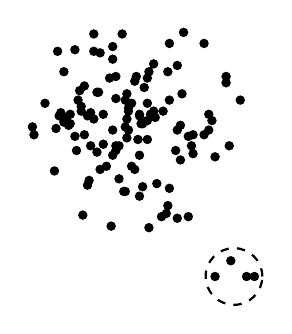
\begin{tikzpicture}[thick,scale=2, every node/.style={scale=5}]
      \fill (1.21, 0.56)  circle (0.3mm) (0.51, 1.02)  circle (0.3mm) (0.61, 1.44)  circle (0.3mm) (0.91, 1.54)  circle (0.3mm) (0.69, 0.58)  circle (0.3mm) (1.2, 1.3)  circle (0.3mm) (1.28, 0.96)  circle (0.3mm) (0.67, 1.21)  circle (0.3mm) (0.34, 0.95)  circle (0.3mm) (0.89, 0.83)  circle (0.3mm) (1.33, 0.38)  circle (0.3mm) (1.3, 1.55)  circle (0.3mm) (1.07, 0.99)  circle (0.3mm) (0.89, 0.62)  circle (0.3mm) (1.07, 0.87)  circle (0.3mm) (0.48, 0.67)  circle (0.3mm) (0.35, 0.9)  circle (0.3mm) (1.26, 1.34)  circle (0.3mm) (0.73, 1.54)  circle (0.3mm) (0.76, 1.17)  circle (0.3mm) (1.02, 1.03)  circle (0.3mm) (1.28, 0.74)  circle (0.3mm) (0.54, 1.3)  circle (0.3mm) (0.73, 1.43)  circle (0.3mm) (0.77, 1.42)  circle (0.3mm) (0.85, 0.93)  circle (0.3mm) (0.97, 1.1)  circle (0.3mm) (1.08, 1.3)  circle (0.3mm) (0.5, 1.43)  circle (0.3mm) (1.25, 0.8)  circle (0.3mm) (1.59, 0.83)  circle (0.3mm) (1.02, 0.51)  circle (0.3mm) (0.79, 0.84)  circle (0.3mm) (1.11, 1.05)  circle (0.3mm) (1.2, 0.45)  circle (0.3mm) (1.66, 1.12)  circle (0.3mm) (0.66, 0.39)  circle (0.3mm) (1.57, 1.27)  circle (0.3mm) (1.19, 0.4)  circle (0.3mm) (0.84, 0.32)  circle (0.3mm) (1.36, 0.9)  circle (0.3mm) (1.21, 1.48)  circle (0.3mm) (1.04, 0.57)  circle (0.3mm) (0.87, 0.83)  circle (0.3mm) (0.92, 0.54)  circle (0.3mm) (0.85, 1.46)  circle (0.3mm) (1.16, 0.38)  circle (0.3mm) (0.94, 0.88)  circle (0.3mm) (1.13, 0.59)  circle (0.3mm) (0.71, 0.83)  circle (0.3mm) (1.26, 0.37)  circle (0.3mm) (1.07, 0.87)  circle (0.3mm) (1.57, 1.23)  circle (0.3mm) (0.62, 0.8)  circle (0.3mm) (1.5, 0.76)  circle (0.3mm) (0.42, 1.1)  circle (0.3mm) (1.43, 1.48)  circle (0.3mm) (1.43, 0.9)  circle (0.3mm) (0.49, 0.94)  circle (0.3mm) (1.08, 0.31)  circle (0.3mm)

      (1.04, 0.97)  circle (0.3mm) (0.95, 0.93)  circle (0.3mm) (1.05, 1.2)  circle (0.3mm) (0.54, 0.98)  circle (0.3mm) (0.71, 1.04)  circle (0.3mm) (0.75, 1.17)  circle (0.3mm) (1.07, 1.26)  circle (0.3mm) (0.63, 1.12)  circle (0.3mm) (0.65, 1.08)  circle (0.3mm) (0.95, 1.05)  circle (0.3mm) (0.83, 1.26)  circle (0.3mm) (0.77, 0.68)  circle (0.3mm) (1.02, 0.77)  circle (0.3mm) (0.64, 1.18)  circle (0.3mm) (0.99, 0.68)  circle (0.3mm) (1.21, 1.12)  circle (0.3mm) (0.75, 0.79)  circle (0.3mm) (1.17, 1.05)  circle (0.3mm) (1.01, 0.87)  circle (0.3mm) (0.69, 1.02)  circle (0.3mm) (1.46, 0.93)  circle (0.3mm) (1.02, 1.02)  circle (0.3mm) (1.26, 0.93)  circle (0.3mm) (1.12, 1.01)  circle (0.3mm) (1.46, 1.03)  circle (0.3mm) (0.93, 0.95)  circle (0.3mm) (0.67, 0.9)  circle (0.3mm) (1.0, 1.27)  circle (0.3mm) (0.99, 1.24)  circle (0.3mm) (0.81, 0.7)  circle (0.3mm) (0.93, 0.54)  circle (0.3mm) (0.97, 0.7)  circle (0.3mm) (0.57, 0.96)  circle (0.3mm) (0.55, 1.01)  circle (0.3mm) (1.33, 0.89)  circle (0.3mm) (0.87, 0.8)  circle (0.3mm) (1.11, 1.35)  circle (0.3mm) (0.85, 1.38)  circle (0.3mm) (0.52, 1.04)  circle (0.3mm) (0.7, 0.61)  circle (0.3mm) (1.48, 0.99)  circle (0.3mm) (1.03, 0.97)  circle (0.3mm) (1.07, 1.1)  circle (0.3mm) (0.65, 1.05)  circle (0.3mm) (0.73, 1.0)  circle (0.3mm) (0.87, 1.13)  circle (0.3mm) (0.87, 1.27)  circle (0.3mm) (1.29, 1.16)  circle (0.3mm) (0.79, 1.03)  circle (0.3mm) (0.94, 1.0)  circle (0.3mm) (0.61, 0.89)  circle (0.3mm) (1.35, 0.83)  circle (0.3mm) (1.36, 0.78)  circle (0.3mm) (0.94, 1.16)  circle (0.3mm) (1.09, 1.03)  circle (0.3mm) (0.85, 0.77)  circle (0.3mm) (0.58, 1.03)  circle (0.3mm) (0.95, 1.07)  circle (0.3mm) (0.58, 0.97)  circle (0.3mm) (0.93, 1.12)  circle (0.3mm);
      \draw[dashed] (1.62,0) circle (1.8mm);
      \fill (1.7,0)  circle (0.3mm) (1.75,0)  circle (0.3mm) (1.5,0)  circle (0.3mm) (1.6,0.1)  circle (0.3mm);
    \end{tikzpicture}};
\end{frame}


\begin{frame}
  \frametitle{Types of Outliers (2)}
  \begin{itemize}
  \item \textbf{\color{airforceblue}Collective} \textbf{outlier}:
    \begin{itemize}
    \item A \textbf{subset} of data objects that collectively \\
      deviates significantly from the whole data set.
    \item Ex.: intrusion detection -- a number of computers \\
      keep sending denial-of-service packages to each other.
    \end{itemize}

  \item \textbf{Detection of collective outliers:}
    \begin{itemize}
    \item Consider not only behavior of individual objects,but also that of groups of objects.
    \item Need to have the background knowledge on the relationship among data objects, such as a distance or similarity measure on objects.
    \end{itemize}
  \item \textbf{A data set may have multiple types of outliers.}
  \item \textbf{One object may belong to more than one type of outlier.}
  \end{itemize}

  \tikzoverlay at (11cm,6cm) {
    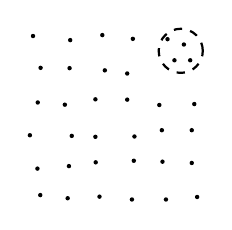
\begin{tikzpicture}[thick,scale=0.4, every node/.style={scale=5}]
      \fill (0.14, 0.02)  circle (0.7mm) (0.05, 0.86)  circle (0.7mm) (-0.19, 1.92)  circle (0.7mm) (0.06, 2.96)  circle (0.7mm) (0.15, 4.06)  circle (0.7mm) (-0.09, 5.07)  circle (0.7mm) (1.01, -0.08)  circle (0.7mm) (1.05, 0.94)  circle (0.7mm) (1.14, 1.9)  circle (0.7mm) (0.92, 2.89)  circle (0.7mm) (1.07, 4.05)  circle (0.7mm) (1.09, 4.94)  circle (0.7mm) (2.02, -0.03)  circle (0.7mm) (1.9, 1.06)  circle (0.7mm) (1.89, 1.87)  circle (0.7mm) (1.89, 3.06)  circle (0.7mm) (2.19, 3.98)  circle 	(0.7mm) (2.11, 5.1)  circle (0.7mm) (3.05, -0.12)  circle (0.7mm) (3.11, 1.11)  circle (0.7mm) (3.13, 1.88)  circle (0.7mm) (2.9, 3.05)  circle (0.7mm) (2.9, 3.88)  circle (0.7mm) (3.08, 4.98)  circle (0.7mm) (4.13, -0.12)  circle (0.7mm) (4.02, 1.08)  circle (0.7mm) (4.0, 2.08)  circle (0.7mm) (3.92, 2.88)  circle (0.7mm) (4.4, 4.3)  circle (0.7mm) (4.18, 4.97)  circle (0.7mm) (5.12, -0.04)  circle (0.7mm) (4.95, 1.04)  circle (0.7mm) (4.95, 2.08)  circle (0.7mm) (5.03, 2.91)  circle (0.7mm) (4.9, 4.3)  circle (0.7mm) (4.7, 4.8)  circle (0.7mm) ;
      \draw[dashed] (4.6,4.6) circle (7mm);
    \end{tikzpicture}};
\end{frame}


\begin{frame}{Challenges of Outlier Detection}
  \begin{itemize}
  \item \textbf{Modeling normal objects and outliers properly.}
    \begin{itemize}
    \item Hard to enumerate all possible normal behaviors in an application.
    \item The border between normal and outlier objects is often a grey area.
    \end{itemize}
  \item \textbf{Application-specific outlier detection.}
    \begin{itemize}
    \item Choice of distance measure among objects and the model of \\
      relationship among objects are application-dependent.
    \item E.g. clinical data: a small deviation could be an outlier; \\
      while in marketing analysis: larger fluctuations.
    \end{itemize}
  \end{itemize}
\end{frame}


\begin{frame}{Challenges of Outlier Detection (II)}
  \begin{itemize}
  \item \textbf{Handling noise in outlier detection.}
    \begin{itemize}
    \item Noise may distort the normal objects and blur the distinction \\
      between normal objects and outliers.
    \item It may hide outliers and reduce the effectiveness of outlier detection.
    \end{itemize}
  \item \textbf{Understandability.}
    \begin{itemize}
    \item Understand why these are outliers: justification of the detection.
    \item Specify the degree of an outlier: \\
      the unlikelihood of the object being generated by a normal mechanism.
    \end{itemize}
  \end{itemize}
\end{frame}
